\chapter{Diskussion}
\label{chap:discussion}

Die in Kapitel \textbf{\ref{chap:existingComponents}} beschriebenen Komponenten Select und Datalist kommen in vielen Webseiten zu Anwendung. 
Das Auswählen eines Wertes aus einer vorgegebenen Menge ist mit diesen Elementen ineffizient und unästhetisch.
Die in Projekt 5 erstellte Länderauswahl löst das Problem aber nur für diesen einen spezifischen Anwendungsfall. 
Die neue Komponente \codestyle{SelectComponent} baut auf der Länderauswahl auf, ist jedoch generalisiert und lässt sich mit unterschiedlichsten Werten anwenden. 
Dabei spielt es keine Rolle, welcher Konstruktor bzw. welche Art der Datenübergabe zur Anwendung kommt. 

Die Datalist und das Select zeigen im UI als auch der Interaktion einige Inkonsistenzen auf. 
Die Darstellung lässt sich mit den wenigen Styling-Möglichkeiten der HTML-Elemente teilweise beheben. 
Richtig unangenehm gestaltet sich die Anwendung dieser Auswahlkomponenten bei einer grossen aber doch begrenzten Menge von Optionen. 
Eine saubere Integration in eine konsistent designte Webseite ist jedoch nicht möglich.
Der Container mit den Werten lässt sich bei beiden Elementen nicht umgestalten und zerstört das Bild des abgestimmten Designs. 
Die Lösungen von Frameworks und Libraries blasen eine ansonsten schlanke Codebasis unnötig auf. 
Zudem bieten diese Komponenten häufig zu viele Funktionen an, welche die Anwendung verkomplizieren. 

An diesem Punkt bietet die \codestyle{SelectComponent} des Kolibri ohne externe Abhängigkeiten eine konsistente und anpassbare Auswahlkomponente an. 
Das Konsistenzproblem ist durch ein klar gestaltetes Design gelöst. 
Die Implementation ist auf den gängisten Browsern Edge (127), Chrome (127), Firefox (128) und Safari (17.5) auf Desktop getestet. 
User-Tests mit Endnutzern zeigen, dass die Komponente dessen Bedürfnisse abdecken und die Auswahl vereinfacht. 
Der modulare Aufbau ermöglicht eine hohe Wiederverwendbarkeit. 
Die Subkomponente \codestyle{ColumnOptionsComponent} kann für ein Einsatzgebiet ausserhalb der Auswahlkomponente zur Anwendung kommen. 
Eine mögliche Verwendung kann bei einer Tabellen-Ansicht sein. 
Ein weiterer Vorteil der einzelnen Komponenten ist, dass andere Projektoren zur Visualisierung zum Einsatz kommen können. 

Diese Arbeit ist zeitlich und personell begrenzt. 
Deswegen bietet die Komponente nur einen Projektor für die Auswahlkomponente. 
Die spät durchgeführten User Tests mit Programmierern führen dazu, dass nach der Implementation der Feedbacks keine zusätzliche Kontrolle mehr durchführbar ist. 
Dies ist als erstes Future Feature im nachfolgenden Kapitel genauer beschrieben. 


\section{Future Features}
\label{sec:future}

Die Zukunft der zwei entstandenen \codestyle{SelectComponent}s zeigt sich sehr vielfältig. 
Durch die modulare Struktur vereinfacht sich die Erweiterung, indem einzelne Komponente wie Projektoren austauschbar sind. 
Nachfolgend sind mögliche Verbesserungen und Features aufgelistet. 


\subsection{Weitergehende User-Tests und Nutzerbefragungen}
\label{sec:moreUserTests}

Die aus den Feedback der Programmierer entstandene \codestyle{SelectComponent} sollte sich weiteren Tests mit Entwicklern stellen. 
Dies garantiert eine gut verständliche Dokumentation und effiziente Einbindung in den Code. 
Allenfalls lassen sich weitere Bugs aufdecken. 
Die weiteren Tests bieten die Möglichkeit einen Vergleich zu den bereits durchgeführten Tests zu ziehen. 
Spezifische Fragen können die Vereinfachung der Anwendung beweisen oder wiederlegen. 

Die Anzahl Personen der Testgruppe massiv zu erhöhen, führt zu mehr Feedback. 
Gewisse Interaktionen der Nutzer können möglicherweise auf bisher unentdeckte Probleme hinweisen. 
Diese lassen sich in einem weiteren Schritt beheben. 

Eine Umfrage bei den Endanwendern weist auf bisher unbekannte Wünsche hin. 
Durch eine grosse Diversität beim Hintergrundwissen der Befragten entstehen neue Designansätze. 
Aus den Feedbacks lassen sich neue Projektoren – ob UI oder Interaktion - designen und umsetzen. 


\subsection{Weitere UI-Projektoren}
\label{sec:moreUi}

Die während des Design-Prozesses entstandenen Prototypen bieten sich als Grundlage für neue UI-Projektoren\footnote{
    Projektoren, die nur die View generieren (ohne Tastatur-Interaktion)
} an. 
Aus diesen Designskizzen lassen sich in Figma ausgearbeitete Prototypen erstellen. 
Diese finden sich in der späteren Implementation zu einzelnen Projektoren wieder. 

Weitere Projektoren könnten den gleichen Aufbau besitzen, aber mit alternativen Design-Implementationen ausgestattet sein. 
Dabei zeigen sich die Unterschiede beispielsweise in der Visualisierung des Highlights, der Cursor Position oder der Selektion. 
Das Desgin kann jedoch wie beim Darkmode die komplette Komponente betreffen. 

Statt einer Spalten-Darstellung visualisiert sich eine Idee als Zeilen-Darstellung (Abbildung \ref{img:futureUi}). 
Die Kategorien zeigen initial nur die ausgewählte Option in einer Zeile an. 
Die \codestyle{ValueOption} stellt die Werte in einer normalen Spalte dar. 
Beim Eintreten\footnote{
    Wechsel der Cursor Position in die Kategorie oder ein Klick auf die Kategorie
} in eine Kategorie ändert sich die Darstellung der aktiven Zeile in ein Rad (Mitte Abbildung \ref{img:futureUi}). 
Sobald das Highlight bzw. die Cursor Position die Kategorie-Zeile verlässt, minimiert sich die Visualisierung zurück auf den selektierten Wert. 
Nach dem Erstellen eines Figma-Prototypen findet sich in dieser Idee ein neuer UI-Projektor wieder. 

\begin{figure}[!htb]
    \centering
    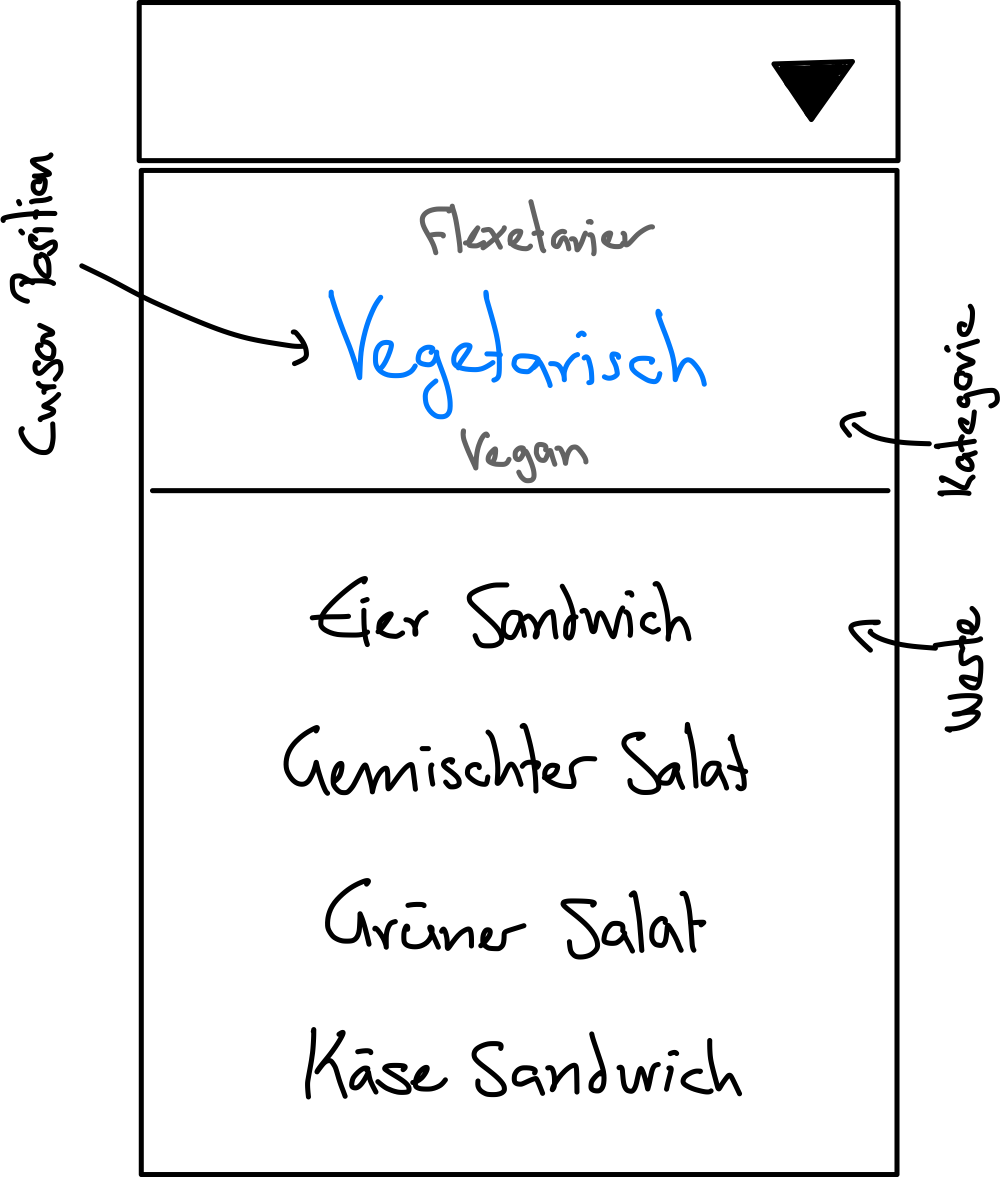
\includegraphics[width=60mm]{future-ui.png}
    \caption{\centering Mögliches UI mit Zeilen-Aufbau}
    \label{img:futureUi}
\end{figure}

Die entstandenen als auch zukünftige UI-Projektoren lassen sich mit unterschiedlichen Interaktionen verbinden. 
Dabei ist es hilfreich, verschiedene Interaktions-Projektoren\footnote{
    Projektoren, die nur die Tastatur-Interaktion definieren
} zu bieten. 


\subsection{Weitere Interaktions-Projektoren}
\label{sec:moreInteraction}

Neue UI-Projektoren lassen sich nicht ausnahmslos mit den bestehenden Tastatur-Inter\-aktionen kombinieren. 
Zudem ist nicht in jeder Situation erwünscht, dass die Cursor Position die Selektion beeinflusst. 
Weitere Projektoren können neue, eventuell UI-Projektor spezifische Interaktionen bieten. 

Ein Interaktions-Projektor kann das Auswahlkomponente bezogene Undo und Redo enthalten. 
Diese Funktion bietet an, eine geänderte Auswahl rückgängig zu machen oder zu wiederholen. 


\subsection{Spezifische Auswahlkomponenten und Erweiterungen}
\label{sec:specificComponents}

Zukünftig besteht die Möglichkeit Auswahlkomponenten für spezielle Anwendungsfälle zu erstellen. 
Ein altbekanntes Beispiel ist die Auswahl eines Datums mit Tag, Monat und Jahr. 
Dabei kann weitere Logik zur Kontrolle der möglichen Werte zum Einsatz kommen. 

Das Erweitern der Multiselect-Funktionalität führt die Anpassung mehrerer Subkomponenten mit sich. 
Es betrifft die Implementation von der \codestyle{SelectComponent} bis hin zu der \codestyle{columnOptionsComponent}. 
Eine mögliche neue Single-Select Komponente bietet die Funktionalität mehrere Kategorien auswählen zu können. 
Hierbei ist zu unterscheiden, ob die ausgewählten Kategorien als \emph{AND}- oder \emph{OR}-Verknüpfung zu verstehen sind. 


\subsection{Performance verbessern und mögliche Datenmenge erhöhen}
\label{sec:betterPerformance}

Die \codestyle{SelectComponent} garantiert bis 5'000 Werte eine annehmbare\footnote{
    Ladezeit < 500ms bis die Webseite fertig geladen ist
} Ladezeit. 
Diese Performance lässt sich weiter optimieren. 
Zudem führen diese Verbesserungen dazu, dass sich eine noch höhere Anzahl Optionen anwenden lässt. 
Eine Kombination der Auswahlkomponente mit der Lazy Table des Kolibri ermöglicht eine optimierte Performance. 
Denn die Lazy Table kann eine Datenmenge von über 100'000 Werte verwalten. 


\subsection{Accessability verbessern}
\label{sec:betterAccessability}

Die entstandene Auswahlkomponente ist nur für nicht beeinträchtigte Menschen optimiert. 
Zukünftig ist die Komponente noch für Screen-Reader und somit für Blinde zu ergänzen. 
Die getroffenen Styles benötigen ein Testing mit Sehbeeinträchtigten, um die Accessability garantieren zu können. 
Dazu zählt zum Beispiel die bekannte Rot-Grün-Schwäche. 


\subsection{Abschliessende Bemerkungen}
\label{sec:endSumup}

All diese Erweiterungen und Verbesserungen zielen darauf ab, die Auswahlkomponente für alle Endnutzer zugänglich zu machen und eine angenehme Benutzung zu ermöglichen. 
Zudem soll die \codestyle{SelectComponent} einfach in jeden bestehenden JavaScript Code einzubinden sein. 
Anschliessend an diese Arbeit steht die Integration in das Toolkit Kolibri an. 
